
\subsection{The Standard Model}
\label{subsec:std_model}


--- \textit{The W-boson }\\
  The most difficult reconstruction of a final state from W decay is the case of a tau lepton. The tau can mimic the signature of hadrons or other leptons in a detector in addition to producing additional missing energy via neutrinos. The tau has a shorter lifetime compared to the other charged leptons and flies a short distance before decaying. If produced from the interaction point in a detector, the tau will travel on average $87\,\mu\text{m}$ before decaying. The other leptons, like the electron, is stable and doesn't decay, and the muon is not stable but is unlikely to decay inside the detector. The tau lepton mainly decays hadronically -- into a tau neutrino and virtual W-boson that produces a pair of quarks. The virtual W's daughter quarks will hadronize into a charged particle ($\pi^\pm$) or radiate more quarks that form either more charged or neutral particles ($\pi^0$). If $\pi^0$'s are created they immediately decay mostly into two photons. When a tau produces a single charged particle this is classified as a 1-prong decay, 3 charged particles is classified as a 3-prong decay. The virtual W in the tau decay is allowed to couple with leptons, so, the tau final state can include either an electron or muon along with the corresponding flavor neutrinos. The decay rates for the tau are given in Table \ref{tab:taudecay}.

\begin{table}
\centering
 \begin{tabular}{|c|l|c|} 
 
 \hline
       & Decay Mode & Branching Ratio  \\ \hline \hline
    Hadronic Modes  & $\pi^- \nu_\tau$  & $10.82\%$  \\
      	($64.79\%$) & $\pi^- \pi^0 \nu_\tau$ & $25.49\%$ \\
     				& $\pi^- \pi^0 \pi^0 \nu_\tau$  & $9.26\%$  \\
     				& $\pi^- \pi^0 \pi^0 \pi^0 \nu_\tau$  & $1.04\%$   \\
      				& $\pi^- \pi^+ \pi^- \nu_\tau$  & $8.99\%$      \\ 
      				& $\pi^- \pi^+ \pi^- \pi^0 \nu_\tau$  & $2.74\%$  \\ \hline
    			    
    Leptonic Modes  & $e^- \nu_e \nu_\tau$ & $17.82\%$   \\
    	($35.21\%$)	& $\mu^- \nu_\mu \nu_\tau $  & $17.39\%$      \\ \midrule \hline
      				
     				
\end{tabular}
        \caption{\label{tab:taudecay}Most common decay modes for the $\tau^-$ lepton \cite{pdg}}
\end{table}
       
  
   

--- \textit {The W Mass}\\
The W-boson is an unstable particle and abides by a total decay rate $\Gamma = 1/\tau$ where $\tau$ is the average lifetime.  A consequence of this decay length is that the observed mass distribution will approximately follow a Breit-Wigner distribution. The mass distribution is centered on the nominal W mass $M_W$ with a width characterized by the full width half maximum $\Gamma_W$. The current highest precision measurement for the mass and width are results of measurements through single $W^\pm$ production. These measurements use the combined results from LEP and Tevatron experiments which reports $M_W = 80.379 \pm 0.012 \, \, \text{GeV} $ and $\Gamma_W = 2.085 \pm 0.042 \,  \,\text{GeV}$ \cite{pdg}. The diagrams representing WW are given in Figure \ref{fig:wwdiag}. The final states of the WW process are either the fully hadronic $WW\rightarrow q\bar{q}q\bar{q}$, semileptonic $WW\rightarrow q\bar{q}\ell\nu_{\ell}$, or fully leptonic $WW\rightarrow \ell \nu \ell \nu$. The semileptonic mode is the most favorable way to measure the W mass because the hadronic system is easily obtained after the identification of the lepton. The hadronic mode is more challenging due to the combinatoric assignment of the four hadronic jets into two W's along with color-reconnection which may cause ``cross-talk" between jets. The leptonic channel is also difficult because of the presence of two neutrinos.


\begin{figure}
\centering
\feynmandiagram [horizontal=a to b] {
  i1 [particle=\(e^{-}\)] -- [fermion] a -- [fermion] i2 [particle=\(e^{+}\)],
  a -- [photon, edge label=\(\gamma / Z\)] b,
  f1 [particle=\(W^{+}\)] -- [photon] b -- [photon] f2 [particle=\(W^{-}\)],
};
    \feynmandiagram[vertical'=a to b ]{
        i1 [particle=\(e^{-}\)]
            -- [fermion] a 
            -- [boson] f1 [particle=\(W^{-}\)],
        a -- [fermion, edge label'=\(\nu\)] b ,
        i2 [particle=\(e^{+}\)]
            -- [anti fermion] b
            -- [boson] f2 [particle=\(W^{+}\)]
    };
\caption{\label{fig:wwdiag} Main WW production modes in the s and t channels. }
\end{figure}

  

\subsection{The Anatomy of an Event}
\label{subsec:collphsx}
--- \textit{Beam effects}\\
Figure \ref{fig:wwdiag} illustrates the production of WW through  $e^- \, e^+$ annihilation. Within the collider annihilation presents two important effects: beamstrahlung and pile-up. The first is related to photons produced from the interactions between the fields of the beams. The radiated photons generally go undetected by escaping down the beam-pipe causing the effective center of mass energy to be reduced at the interaction point. There is a significant probability that these photons will interact with other photons or beam particles and produce hadrons that scatter into the detector and mix in with the event of interest. These particles add a source of confusion wherein the foreign particles ``pile-up"  ontop of the true particles of an event, thus  trying to resolve the true particles of the event becomes more challenging. 

--- \textit{Helicity}\\
The second underlying physics property in every event is related to the helicity(spin) of the interacting electron and positron. There are four possible combinations of electron and positron helicities where each initial particle is either left or right handed. More explicitly, a collision can consist of  $e^-_L e^+_R$(LR) with left-handed electron and right-handed positron , $e^-_R e^+_L$(RL)  with right handed electron and left handed positron, or mirroring helicities RR and LL.  The beams in the collider are mixed with multiple helicities which is represented by overall partial longitudinal beam polarizations $P_{e^-} \, P_{e^+}$. A diagram of possible tree-level spin configuration is shown in Figure \ref{fig:spindiag}. In the s-channel, the electron positron helicities  are directly coupled, therefore, two W-bosons can only be produced in LR and RL configurations, whereas in the mirrored configuration the  recombination into particle of spin 1 is  not possible. In the t-channel diagrams, the W's are directly coupled to the beam particles. The W has pure coupling only to left handed electrons or right handed positrons so the number of  WW events produced are sensitive to the beam polarization\cite{thomson}.  If the number of events produced is sensitive to polarization then the overall cross-section for WW production is sensitive to beam polarization. 

\begin{figure}

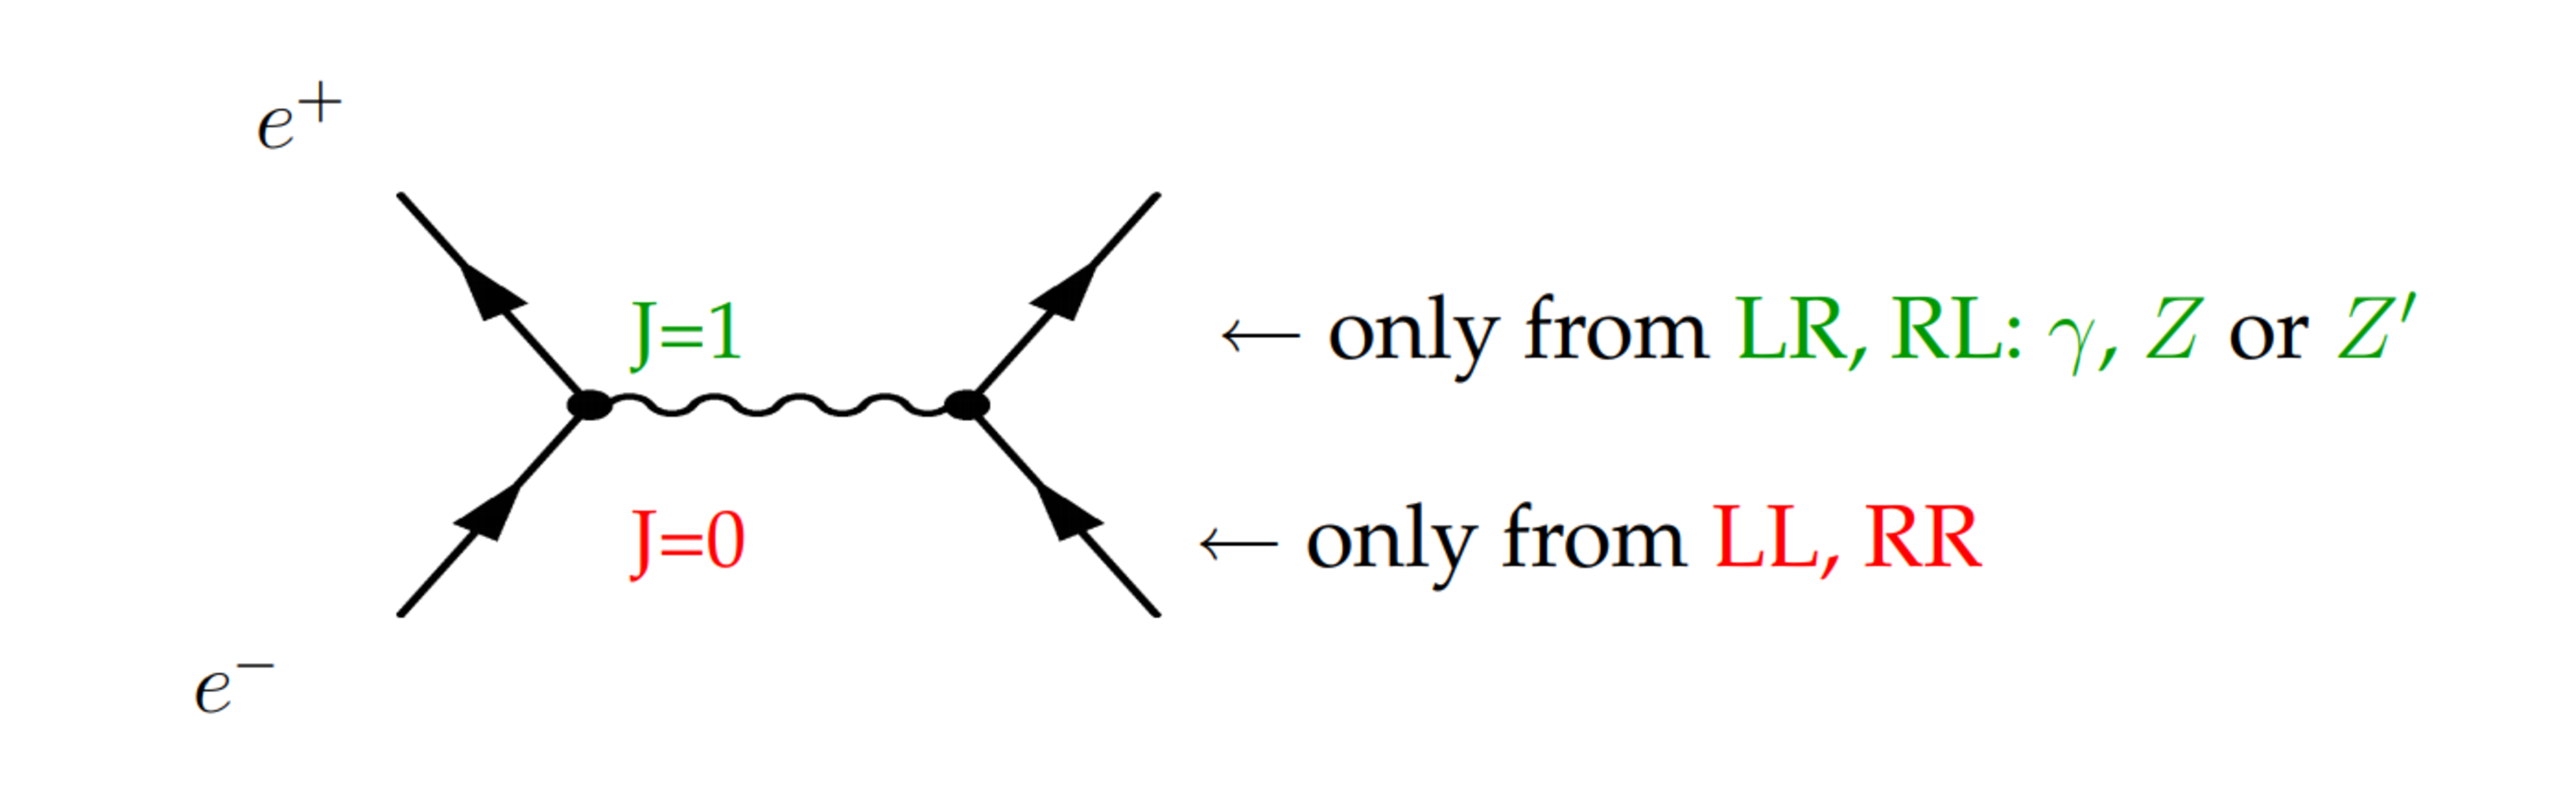
\includegraphics[width=0.49\textwidth]{helicity1.pdf}
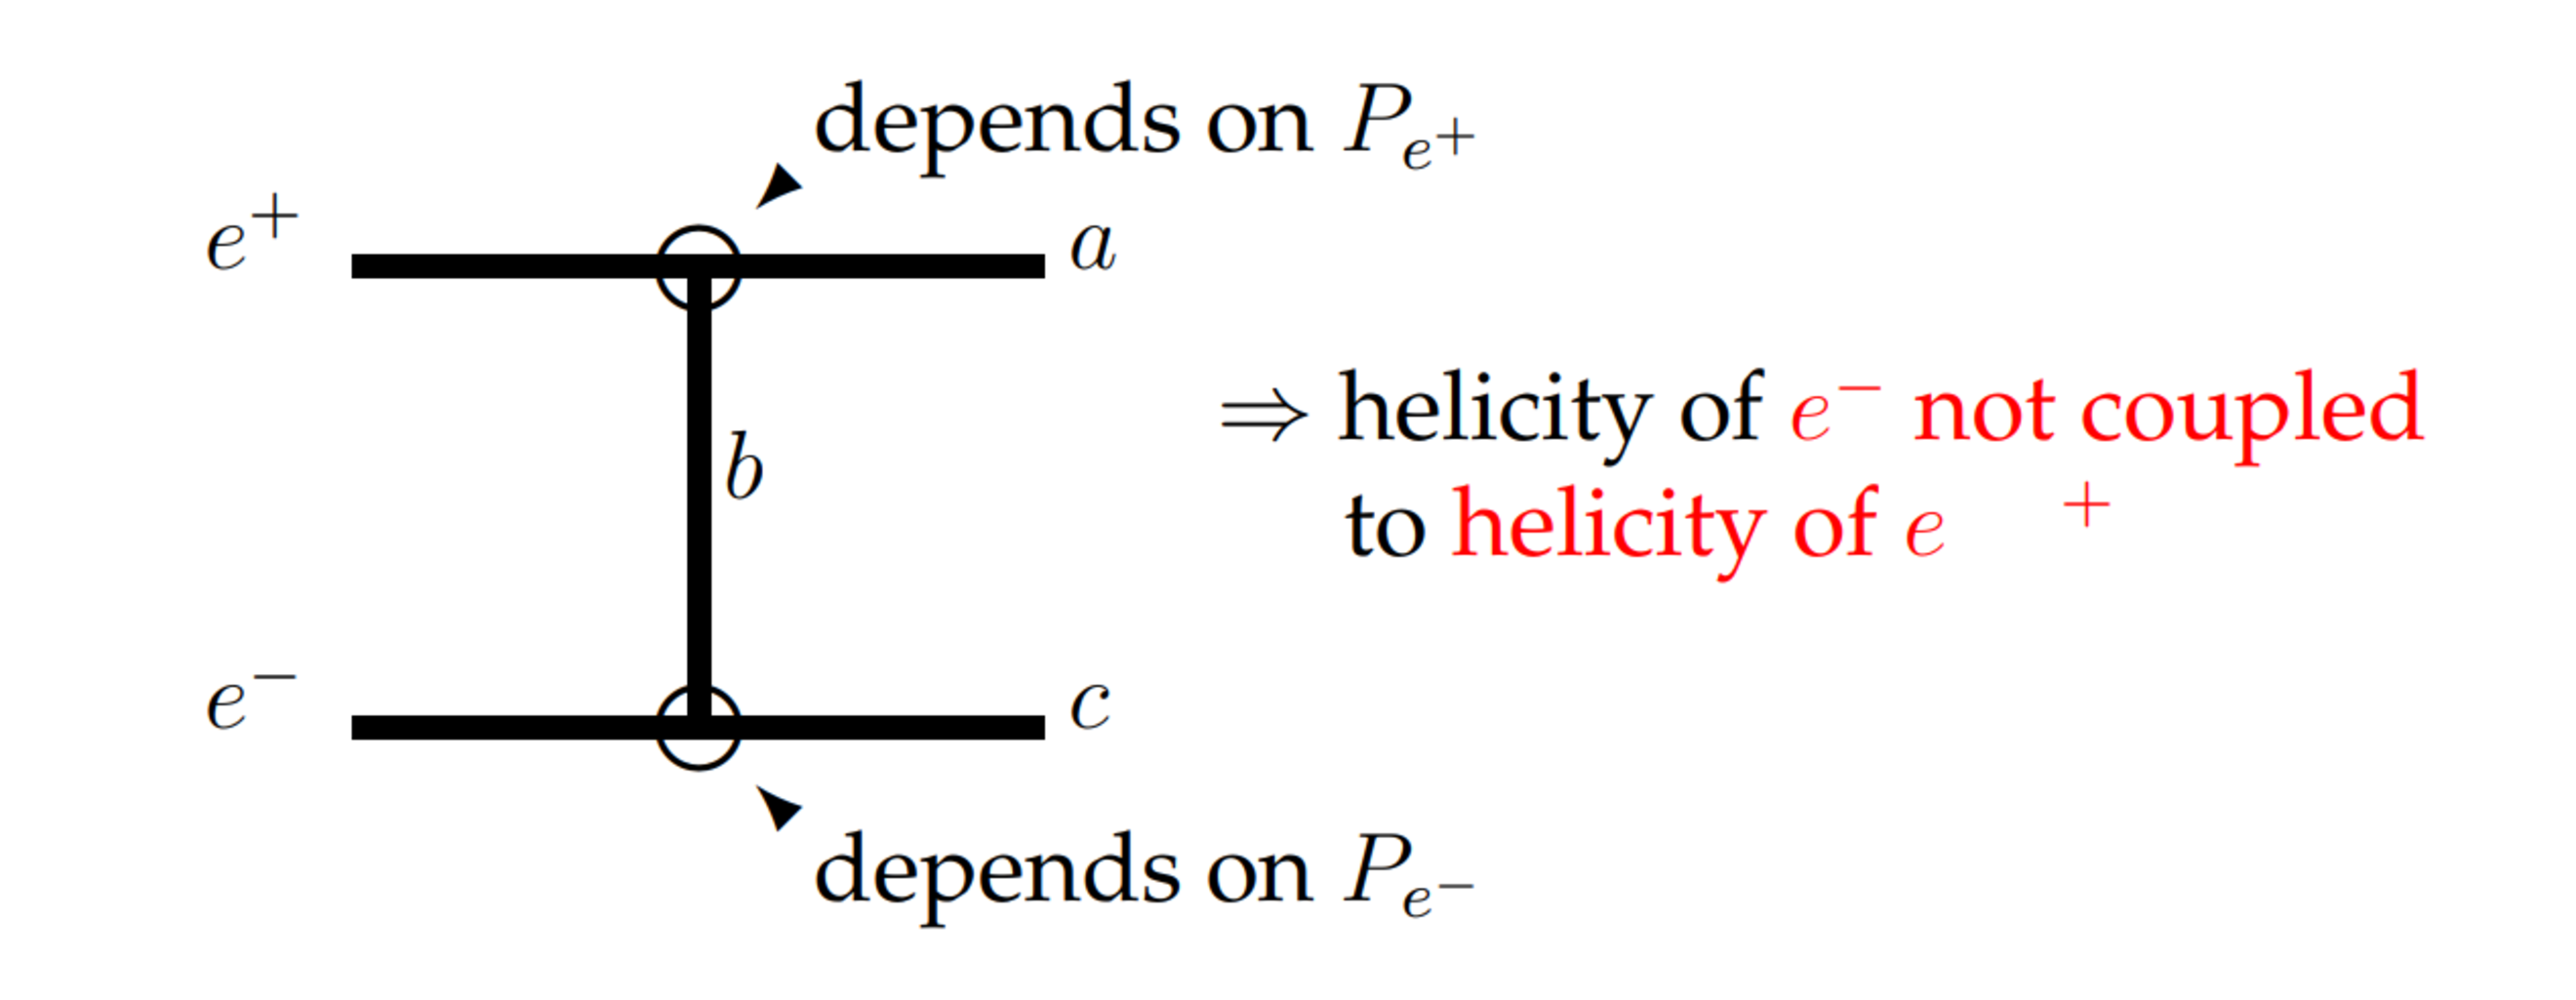
\includegraphics[width=0.49\textwidth]{helicity2.pdf}
\caption{Possible spin configurations in the s and t channel. \cite{helicity}}
\label{fig:spindiag}
\end{figure}


--- \textit{Cross-section}\\
The cross-section is an important measurement because it verifies consistency with the underlying standard model predictions for the rate at which a process occurs. This measurement is doubly important for the WW process because it implicitly provides an in situ measurement of the beam polarizations. By definition, the cross-section is a cross-sectional area and represents the probability of an interaction. The total number of events $N$ observed for a process is given by $ N= \sigma L$ with the cross-section denoted by $\sigma$ and $L$ is the integrated luminosity which is a measure of the total number of collisions. In a physics analysis the desired process(signal) is accompanied by other processes(background) that can unfortunately not be clearlly distinguished from the signal events. Topological or kinematic cuts are applied to each event to minimize the contamination of background events that enter the signal region when trying to count the number of signal events. This reduces the number of observed events $N$ by the number of events lost to the event selection criteria. Thus the number of events observed is then 
\begin{equation}
N = \sigma  L  \epsilon
\end{equation}
where $\epsilon$ is the efficiency of the signal selection in Monte Carlo simulation. The signal efficiency is defined as:
 \begin{equation}
\epsilon = \frac{\text{The number of signal events that pass selection}}{ \text{The total number of signal events that can be selected}}
\end{equation} 
One thing to note is that for a specific process the cross-section includes contributions from all Feynman diagrams that have the same initial and final state particles. This includes diagrams that are essentially not ``signal-like". For WW, examples of these contributing diagrams are given in Figure \ref{fig:offshell}.

\begin{figure}
\begin{fmffile}{feyngraph}
\parbox{0.3\textwidth}{
\begin{fmfgraph*}(85,75)
\fmflabel{\sm$e^+ $}{v 16}
\fmf{fermion}{v 20,v 16}
\fmflabel{\sm$e^+ $}{v  4}
\fmf{fermion}{v  4,v 20}
\fmf{boson,lab=\sm\cyan$\gamma$}{v 21,v 20}
\fmflabel{\sm$\bar{u} $}{v  1}
\fmf{fermion}{v  1,v 21}
\fmf{fermion,lab=\sm\cyan$\bar{u}$}{v 21,v 23}
\fmflabel{\sm$d\ $}{v  2}
\fmf{fermion}{v 23,v  2}
\fmf{boson,lab=\sm\cyan$W^-$}{v 23,v  0}
\fmflabel{\sm$\nu_e $}{v  8}
\fmf{fermion}{v  0,v  8}
\fmflabel{\sm$e^- $}{v 32}
\fmf{fermion}{v 32,v  0}
\fmfleft{v 16,v 32}
\fmfright{v  4,v  1,v  2,v  8}
\end{fmfgraph*}\\ 
} \quad \parbox{0.3\textwidth}{
\begin{fmfgraph*}(100,75)
\fmflabel{\sm$e^+ $}{v 16}
\fmf{fermion}{v  0,v 16}
\fmflabel{\sm$\nu_\mu $}{v  8}
\fmf{fermion}{v 11,v  8}
\fmflabel{\sm$\bar{u} $}{v  1}
\fmf{fermion}{v  1,v  3}
\fmflabel{\sm$d $}{v  2}
\fmf{fermion}{v  3,v  2}
\fmf{boson,lab=\sm\blue$W^-$}{v  3,v 11}
\fmf{fermion}{v 15,v 11}
\fmflabel{\sm$\mu^+$}{v  4}
\fmf{fermion}{v  4,v 15}
\fmf{boson,lab=\sm\blue$Z$}{v  0,v 15}
\fmflabel{\sm$e^- $}{v 32}
\fmf{fermion}{v 32,v  0}
\fmfleft{v 16,v 32}
\fmfright{v  8,v  1,v  2,v  4}
\end{fmfgraph*}\\
}\quad \parbox{0.3\textwidth}{
\begin{fmfgraph*}(85,75)
\fmflabel{\sm$e^+$}{v 16}
\fmf{fermion}{v 27,v 16}
\fmflabel{\sm$\bar\nu_e$}{v  8}
\fmf{fermion}{v  8,v 11}
\fmflabel{\sm$u$}{v  1}
\fmf{fermion}{v  3,v  1}
\fmflabel{\sm$\bar{d}$}{v  2}
\fmf{fermion}{v  2,v  3}
\fmf{boson,lab=\sm\blue$W^+$}{v 11,v  3}
\fmf{fermion}{v 11,v 27}
\fmf{boson,lab=\sm\cyan$\gamma$}{v  0,v 27}
\fmflabel{\sm$e^-$}{v  4}
\fmf{fermion}{v  0,v  4}
\fmflabel{\sm$e^-$}{v 32}
\fmf{fermion}{v 32,v  0}
\fmfleft{v 16,v 32}
\fmfright{v  8,v  1,v  2,v  4}
\end{fmfgraph*}\\

}

\end{fmffile}
\caption{Non signal-like contributions to the WW cross-section, such that, a pair of final state particles are not constrained to the W mass distribution. The right-most diagram shows the electron channel dominant contribution to mirrored initial state helicites and gives a significant boost to the overall WW cross-section in the $e$ channel.  }
\label{fig:offshell}
\end{figure}




